\documentclass[12pt]{standalone}

\usepackage{tikz}

\begin{document}

\tikzset{every picture/.style={line width=0.75pt}} %set default line width to 0.75pt        

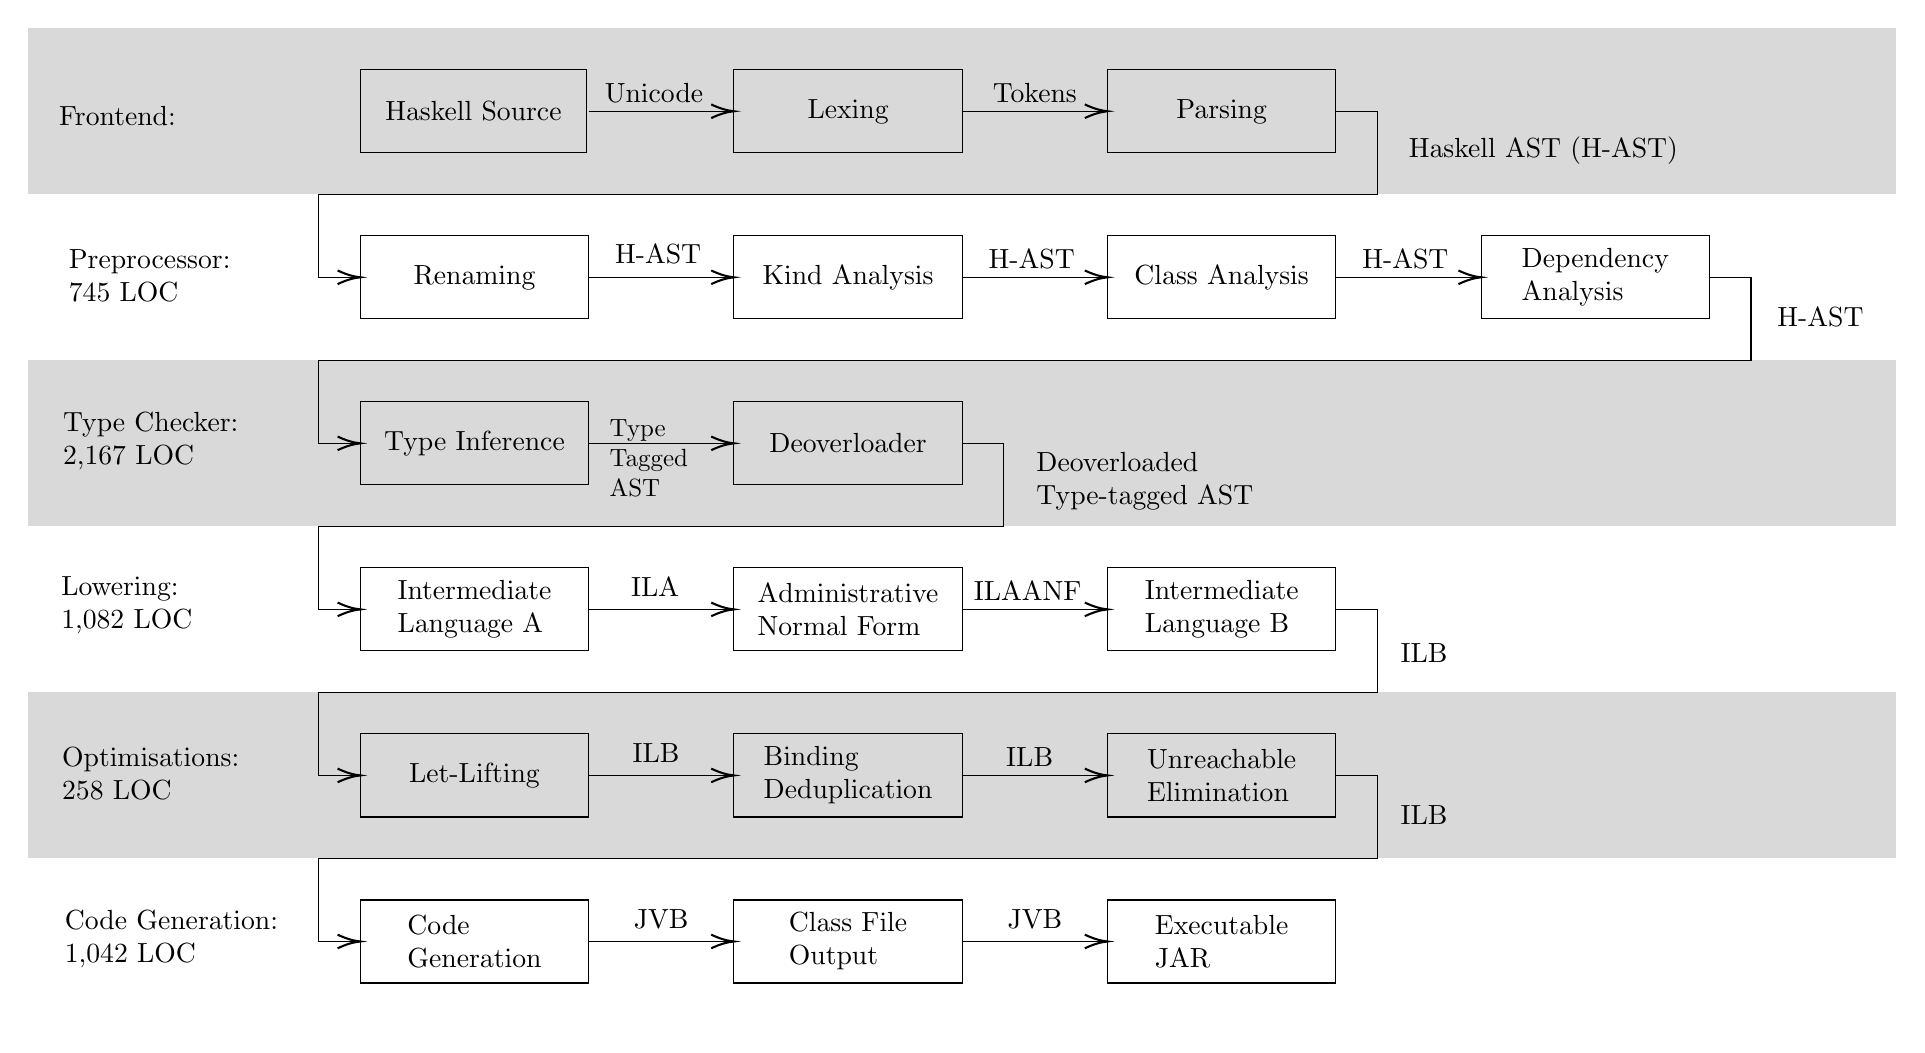
\begin{tikzpicture}[x=0.75pt,y=0.75pt,yscale=-1,xscale=1]
%uncomment if require: \path (0,494); %set diagram left start at 0, and has height of 494

%Shape: Rectangle [id:dp2839023142731987] 
\draw   (160.09,30) -- (268.91,30) -- (268.91,70) -- (160.09,70) -- cycle ;

%Shape: Rectangle [id:dp06804606171058702] 
\draw   (340,30) -- (450,30) -- (450,70) -- (340,70) -- cycle ;

%Shape: Rectangle [id:dp3961237870791873] 
\draw   (520,30) -- (630,30) -- (630,70) -- (520,70) -- cycle ;

%Straight Lines [id:da6049104803203251] 
\draw    (450,50) -- (518,50) ;
\draw [shift={(520,50)}, rotate = 180] [color={rgb, 255:red, 0; green, 0; blue, 0 }  ][line width=0.75]    (10.93,-3.29) .. controls (6.95,-1.4) and (3.31,-0.3) .. (0,0) .. controls (3.31,0.3) and (6.95,1.4) .. (10.93,3.29)   ;

%Straight Lines [id:da275664841754533] 
\draw    (270,50) -- (338,50) ;
\draw [shift={(340,50)}, rotate = 180] [color={rgb, 255:red, 0; green, 0; blue, 0 }  ][line width=0.75]    (10.93,-3.29) .. controls (6.95,-1.4) and (3.31,-0.3) .. (0,0) .. controls (3.31,0.3) and (6.95,1.4) .. (10.93,3.29)   ;

%Straight Lines [id:da7039279955126092] 
\draw    (630,50) -- (650,50) -- (650,90) -- (140,90) -- (140,130) -- (158,130) ;
\draw [shift={(160,130)}, rotate = 180] [color={rgb, 255:red, 0; green, 0; blue, 0 }  ][line width=0.75]    (10.93,-3.29) .. controls (6.95,-1.4) and (3.31,-0.3) .. (0,0) .. controls (3.31,0.3) and (6.95,1.4) .. (10.93,3.29)   ;

%Shape: Rectangle [id:dp47701841006319756] 
\draw   (160,110) -- (270,110) -- (270,150) -- (160,150) -- cycle ;

%Shape: Rectangle [id:dp08823880355784341] 
\draw   (340,110) -- (450,110) -- (450,150) -- (340,150) -- cycle ;

%Shape: Rectangle [id:dp9014362795354506] 
\draw   (520,110) -- (630,110) -- (630,150) -- (520,150) -- cycle ;

%Shape: Rectangle [id:dp6611555253977356] 
\draw   (700,110) -- (810,110) -- (810,150) -- (700,150) -- cycle ;

%Straight Lines [id:da7123909003841777] 
\draw    (270,130) -- (338,130) ;
\draw [shift={(340,130)}, rotate = 180] [color={rgb, 255:red, 0; green, 0; blue, 0 }  ][line width=0.75]    (10.93,-3.29) .. controls (6.95,-1.4) and (3.31,-0.3) .. (0,0) .. controls (3.31,0.3) and (6.95,1.4) .. (10.93,3.29)   ;

%Straight Lines [id:da7870660676764617] 
\draw    (450,130) -- (518,130) ;
\draw [shift={(520,130)}, rotate = 180] [color={rgb, 255:red, 0; green, 0; blue, 0 }  ][line width=0.75]    (10.93,-3.29) .. controls (6.95,-1.4) and (3.31,-0.3) .. (0,0) .. controls (3.31,0.3) and (6.95,1.4) .. (10.93,3.29)   ;

%Straight Lines [id:da0035759925395427716] 
\draw    (630,130) -- (698,130) ;
\draw [shift={(700,130)}, rotate = 180] [color={rgb, 255:red, 0; green, 0; blue, 0 }  ][line width=0.75]    (10.93,-3.29) .. controls (6.95,-1.4) and (3.31,-0.3) .. (0,0) .. controls (3.31,0.3) and (6.95,1.4) .. (10.93,3.29)   ;

%Straight Lines [id:da4775390405469113] 
\draw    (810,130) -- (830,130) -- (830,170) -- (140,170) -- (140,210) -- (158,210) ;
\draw [shift={(160,210)}, rotate = 180] [color={rgb, 255:red, 0; green, 0; blue, 0 }  ][line width=0.75]    (10.93,-3.29) .. controls (6.95,-1.4) and (3.31,-0.3) .. (0,0) .. controls (3.31,0.3) and (6.95,1.4) .. (10.93,3.29)   ;

%Shape: Rectangle [id:dp40116429363803907] 
\draw   (160,190) -- (270,190) -- (270,230) -- (160,230) -- cycle ;

%Shape: Rectangle [id:dp5949915799358637] 
\draw   (340,190) -- (450,190) -- (450,230) -- (340,230) -- cycle ;

%Shape: Rectangle [id:dp8755038003246715] 
\draw   (160,270) -- (270,270) -- (270,310) -- (160,310) -- cycle ;

%Shape: Rectangle [id:dp6976399039028177] 
\draw   (340,270) -- (450,270) -- (450,310) -- (340,310) -- cycle ;

%Shape: Rectangle [id:dp2467611390093658] 
\draw   (520,270) -- (630,270) -- (630,310) -- (520,310) -- cycle ;

%Straight Lines [id:da6672689880773601] 
\draw    (270,210) -- (338,210) ;
\draw [shift={(340,210)}, rotate = 180] [color={rgb, 255:red, 0; green, 0; blue, 0 }  ][line width=0.75]    (10.93,-3.29) .. controls (6.95,-1.4) and (3.31,-0.3) .. (0,0) .. controls (3.31,0.3) and (6.95,1.4) .. (10.93,3.29)   ;

%Straight Lines [id:da7387567305722836] 
\draw    (270,290) -- (338,290) ;
\draw [shift={(340,290)}, rotate = 180] [color={rgb, 255:red, 0; green, 0; blue, 0 }  ][line width=0.75]    (10.93,-3.29) .. controls (6.95,-1.4) and (3.31,-0.3) .. (0,0) .. controls (3.31,0.3) and (6.95,1.4) .. (10.93,3.29)   ;

%Straight Lines [id:da6168610047888969] 
\draw    (450,290) -- (518,290) ;
\draw [shift={(520,290)}, rotate = 180] [color={rgb, 255:red, 0; green, 0; blue, 0 }  ][line width=0.75]    (10.93,-3.29) .. controls (6.95,-1.4) and (3.31,-0.3) .. (0,0) .. controls (3.31,0.3) and (6.95,1.4) .. (10.93,3.29)   ;

%Straight Lines [id:da5214550901341647] 
\draw    (450,210) -- (470,210) -- (470,250) -- (140,250) -- (140,290) -- (158,290) ;
\draw [shift={(160,290)}, rotate = 180] [color={rgb, 255:red, 0; green, 0; blue, 0 }  ][line width=0.75]    (10.93,-3.29) .. controls (6.95,-1.4) and (3.31,-0.3) .. (0,0) .. controls (3.31,0.3) and (6.95,1.4) .. (10.93,3.29)   ;

%Straight Lines [id:da229095719480627] 
\draw    (630,290) -- (650,290) -- (650,330) -- (140,330) -- (140,370) -- (158,370) ;
\draw [shift={(160,370)}, rotate = 180] [color={rgb, 255:red, 0; green, 0; blue, 0 }  ][line width=0.75]    (10.93,-3.29) .. controls (6.95,-1.4) and (3.31,-0.3) .. (0,0) .. controls (3.31,0.3) and (6.95,1.4) .. (10.93,3.29)   ;

%Shape: Rectangle [id:dp9595115062366888] 
\draw   (160,350) -- (270,350) -- (270,390) -- (160,390) -- cycle ;

%Shape: Rectangle [id:dp6366072891095023] 
\draw   (340,350) -- (450,350) -- (450,390) -- (340,390) -- cycle ;

%Shape: Rectangle [id:dp14041439244406329] 
\draw   (520,350) -- (630,350) -- (630,390) -- (520,390) -- cycle ;

%Shape: Rectangle [id:dp00899066638233359] 
\draw   (160,430) -- (270,430) -- (270,470) -- (160,470) -- cycle ;

%Shape: Rectangle [id:dp5714224272730245] 
\draw   (340,430) -- (450,430) -- (450,470) -- (340,470) -- cycle ;

%Shape: Rectangle [id:dp38690758901200883] 
\draw   (520,430) -- (630,430) -- (630,470) -- (520,470) -- cycle ;

%Straight Lines [id:da1521242365631067] 
\draw    (630,370) -- (650,370) -- (650,410) -- (140,410) -- (140,450) -- (158,450) ;
\draw [shift={(160,450)}, rotate = 180] [color={rgb, 255:red, 0; green, 0; blue, 0 }  ][line width=0.75]    (10.93,-3.29) .. controls (6.95,-1.4) and (3.31,-0.3) .. (0,0) .. controls (3.31,0.3) and (6.95,1.4) .. (10.93,3.29)   ;

%Straight Lines [id:da4349746435709425] 
\draw    (270,370) -- (338,370) ;
\draw [shift={(340,370)}, rotate = 180] [color={rgb, 255:red, 0; green, 0; blue, 0 }  ][line width=0.75]    (10.93,-3.29) .. controls (6.95,-1.4) and (3.31,-0.3) .. (0,0) .. controls (3.31,0.3) and (6.95,1.4) .. (10.93,3.29)   ;

%Straight Lines [id:da11627829926648625] 
\draw    (450,370) -- (518,370) ;
\draw [shift={(520,370)}, rotate = 180] [color={rgb, 255:red, 0; green, 0; blue, 0 }  ][line width=0.75]    (10.93,-3.29) .. controls (6.95,-1.4) and (3.31,-0.3) .. (0,0) .. controls (3.31,0.3) and (6.95,1.4) .. (10.93,3.29)   ;

%Straight Lines [id:da42866908441112306] 
\draw    (270,450) -- (338,450) ;
\draw [shift={(340,450)}, rotate = 180] [color={rgb, 255:red, 0; green, 0; blue, 0 }  ][line width=0.75]    (10.93,-3.29) .. controls (6.95,-1.4) and (3.31,-0.3) .. (0,0) .. controls (3.31,0.3) and (6.95,1.4) .. (10.93,3.29)   ;

%Straight Lines [id:da6859077813878957] 
\draw    (450,450) -- (518,450) ;
\draw [shift={(520,450)}, rotate = 180] [color={rgb, 255:red, 0; green, 0; blue, 0 }  ][line width=0.75]    (10.93,-3.29) .. controls (6.95,-1.4) and (3.31,-0.3) .. (0,0) .. controls (3.31,0.3) and (6.95,1.4) .. (10.93,3.29)   ;

%Shape: Rectangle [id:dp6792340646900928] 
\draw  [draw opacity=0][fill={rgb, 255:red, 0; green, 0; blue, 0 }  ,fill opacity=0.15 ] (0,10) -- (900,10) -- (900,90) -- (0,90) -- cycle ;
%Shape: Rectangle [id:dp4662108386005053] 
\draw  [draw opacity=0][fill={rgb, 255:red, 0; green, 0; blue, 0 }  ,fill opacity=0.15 ] (0,170) -- (900,170) -- (900,250) -- (0,250) -- cycle ;
%Shape: Rectangle [id:dp5379997899832005] 
\draw  [draw opacity=0][fill={rgb, 255:red, 0; green, 0; blue, 0 }  ,fill opacity=0.15 ] (0,330) -- (900,330) -- (900,410) -- (0,410) -- cycle ;
%Shape: Rectangle [id:dp6071848931069018] 
\draw  [draw opacity=0] (0,90) -- (900,90) -- (900,170) -- (0,170) -- cycle ;
%Shape: Rectangle [id:dp33144369494693293] 
\draw  [draw opacity=0] (0,250) -- (900,250) -- (900,330) -- (0,330) -- cycle ;
%Shape: Rectangle [id:dp32824444371126216] 
\draw  [draw opacity=0] (0,410) -- (900,410) -- (900,490) -- (0,490) -- cycle ;

% Text Node
\draw (214.5,50) node  [align=left] {Haskell Source};
% Text Node
\draw (43,52) node  [align=left] {Frontend:};
% Text Node
\draw (395,50) node  [align=left] {Lexing};
% Text Node
\draw (575,50) node  [align=left] {Parsing};
% Text Node
\draw (301.5,41) node  [align=left] {Unicode};
% Text Node
\draw (485,41) node  [align=left] {Tokens};
% Text Node
\draw (215,130) node  [align=left] {Renaming};
% Text Node
\draw (395,130) node  [align=left] {Kind Analysis};
% Text Node
\draw (575,130) node  [align=left] {Class Analysis};
% Text Node
\draw (755,130) node  [align=left] {Dependency\\Analysis};
% Text Node
\draw (730,69) node  [align=left] {Haskell AST (H-AST)};
% Text Node
\draw (58.5,129) node  [align=left] {Preprocessor:\\745 LOC};
% Text Node
\draw (303.5,119) node  [align=left] {H-AST};
% Text Node
\draw (483.5,121) node  [align=left] {H-AST};
% Text Node
\draw (663.5,121) node  [align=left] {H-AST};
% Text Node
\draw (215,210) node  [align=left] {Type Inference};
% Text Node
\draw (395,210) node  [align=left] {Deoverloader};
% Text Node
\draw (215,290) node  [align=left] {Intermediate\\Language A};
% Text Node
\draw (395,290) node  [align=left] {Administrative\\Normal Form};
% Text Node
\draw (575,290) node  [align=left] {Intermediate\\Language B};
% Text Node
\draw (59,209) node  [align=left] {Type Checker:\\2,167 LOC};
% Text Node
\draw (47.5,288) node  [align=left] {Lowering:\\1,082 LOC};
% Text Node
\draw (863.5,149) node  [align=left] {H-AST};
% Text Node
\draw (299,217) node [scale=0.9] [align=left] {Type\\Tagged\\AST};
% Text Node
\draw (538,228) node  [align=left] {Deoverloaded\\Type-tagged AST};
% Text Node
\draw (302,279) node  [align=left] {ILA};
% Text Node
\draw (481.5,281) node  [align=left] {ILAANF};
% Text Node
\draw (215,370) node  [align=left] {Let-Lifting};
% Text Node
\draw (395,370) node  [align=left] {Binding\\Deduplication};
% Text Node
\draw (575,370) node  [align=left] {Unreachable\\Elimination};
% Text Node
\draw (215,450) node  [align=left] {Code\\Generation};
% Text Node
\draw (395,450) node  [align=left] {Class File\\Output};
% Text Node
\draw (575,450) node  [align=left] {Executable\\JAR};
% Text Node
\draw (59,369) node  [align=left] {Optimisations:\\258 LOC};
% Text Node
\draw (69,449) node  [align=left] {Code Generation:\\1,042 LOC};
% Text Node
\draw (302.5,359) node  [align=left] {ILB};
% Text Node
\draw (482.5,361) node  [align=left] {ILB};
% Text Node
\draw (672.5,311) node  [align=left] {ILB};
% Text Node
\draw (672.5,389) node  [align=left] {ILB};
% Text Node
\draw (305,439) node  [align=left] {JVB};
% Text Node
\draw (485,439) node  [align=left] {JVB};


\end{tikzpicture}

\end{document}